%%% Local Variables:
%%% coding: utf-8
%%% mode: latex
%%% TeX-engine: xetex
%%% End:
\documentclass[10pt]{beamer}
% NOTE May need to manually set tex engine in emacs

\usetheme[progressbar=frametitle]{metropolis}
\usepackage{appendixnumberbeamer}

\usepackage{svg}
\usepackage{ulem}
\usepackage{cancel}

\usepackage{pifont}
\newcommand{\cmark}{\ding{51}}
\newcommand{\xmark}{\ding{55}}

\usepackage[dvipsnames]{xcolor}
\definecolor{mLightGreen}{HTML}{14B03D}

\usepackage{booktabs}
\usepackage[scale=2]{ccicons}

\usepackage{graphicx}

\usepackage{pgfplots}
\usepgfplotslibrary{dateplot}

\usepackage{todonotes}
\newif\ifdraft
\drafttrue
\newcommand{\todoin}[1]{\ifdraft{\todo[inline]{TODO:\@ #1}}\fi}

\usepackage{xspace}
\usepackage{mathpartir}
\newcommand{\themename}{\textbf{\textsc{metropolis}}\xspace}

\newcommand{\Set}{\mathbf{Set}}
\newcommand{\String}{\mathbf{String}}

\usetikzlibrary{automata, positioning, arrows, fit}
\tikzset{
  invisible/.style={opacity=0},
  visible on/.style={alt={#1{}{invisible}}},
  alt/.code args={<#1>#2#3}{%
    \alt<#1>{\pgfkeysalso{#2}}{\pgfkeysalso{#3}} % \pgfkeysalso doesn't change the path
  },
}
\usepackage{jigsaw}


\title{\Huge Formal Grammars as Types \\ \large in Non-commutative Linear-non-linear Type Theory}
\date{\today}
\author{Steven Schaefer}
\institute{University of Michigan}
% \titlegraphic{
\includegraphics[height=1.5cm]{figures/umich.png}}
%

% \usepackage[backend=bibtex]{biblatex}
% \addbibresource{refs}

\begin{document}

\maketitle

\metroset{block=fill}

% \begin{frame}{Table of Contents}
%   \setbeamertemplate{section in toc}[sections numbered]
%   \tableofcontents[hideallsubsections]
% \end{frame}

% \section{Introduction}

% \begin{frame}{Software is Buggy!}
%   % \begin{figure}
%   % 
\includegraphics[scale=0.5]{figures/bugs.jpeg}
%   % \end{figure} \pause

%   \todoin{Put a good meme here or smth}
% \end{frame}

\begin{frame}{Compilers: Do They Work?}
  \begin{center}
  \begin{tikzpicture}[node distance=3.7cm]
    \node (sourceCode) [visible on=<2->] {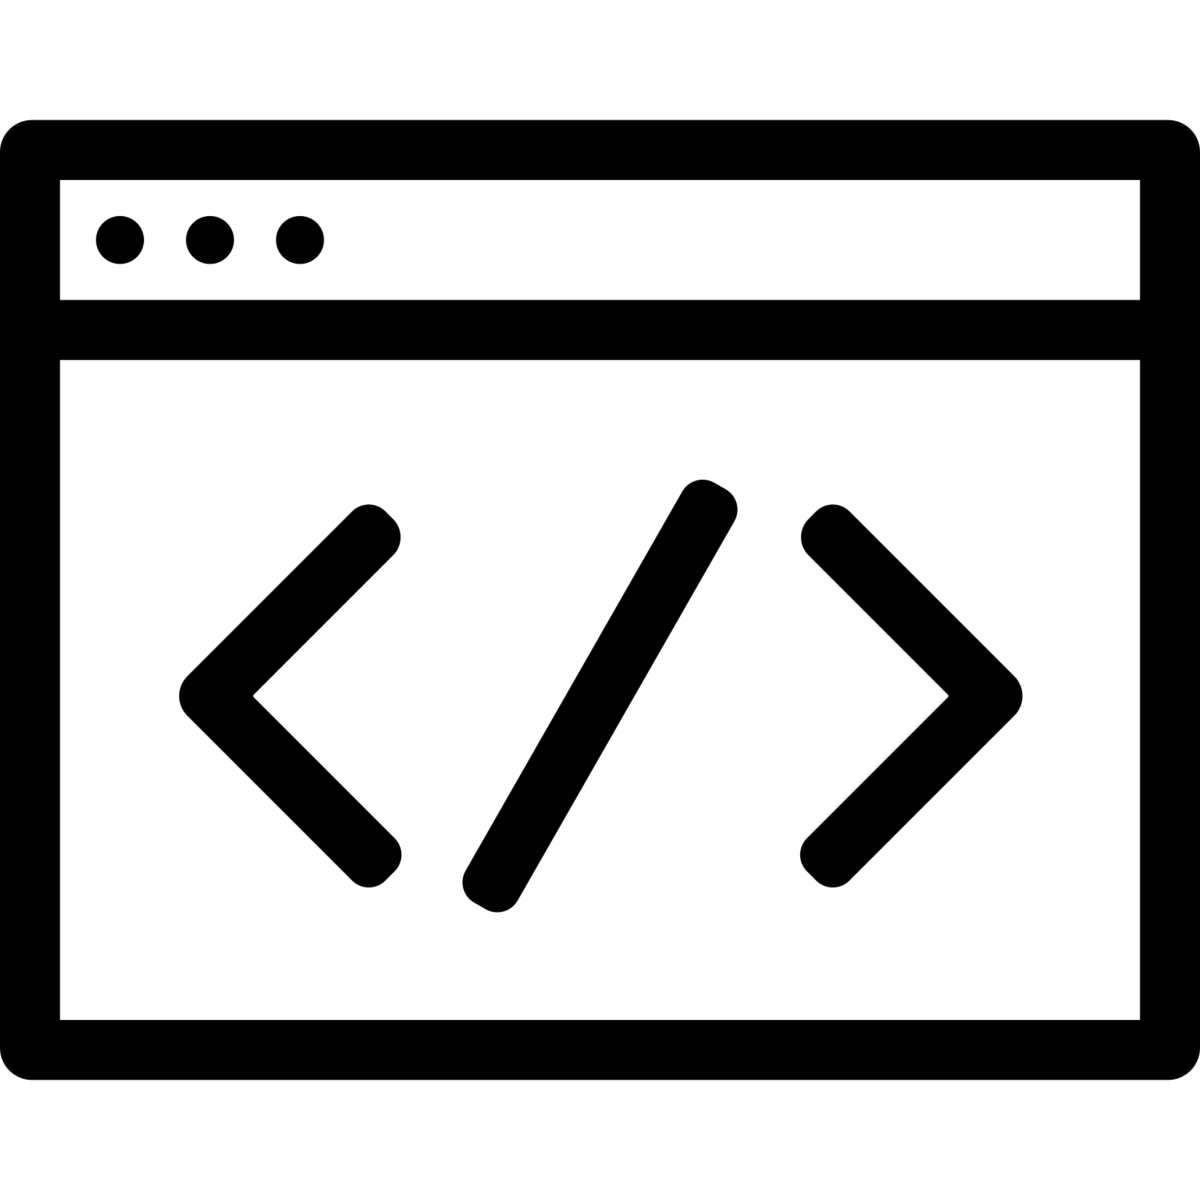
\includegraphics[width=2cm]{figures/srccode.png}};
    \node (srcLabel) [above=-0.3cm of sourceCode,visible on=<2->] {Source Code};
    \node (compiler) [right of=sourceCode, visible on=<1->] {
\includegraphics[width=1cm]{figures/c.png}};
    \node (compilerLabel) [above=-0.3cm of compiler, visible on=<1->] {C Compiler};
    \node (outputCode) [right of=compiler, visible on=<3->] {
\includegraphics[width=2.5cm]{figures/binary.png}};
    \node (outputLabel) [above=-0.55cm of outputCode, visible on=<3->] {Machine Code};


    \draw [->, thick, visible on=<2->, shorten >= 0.6cm] (sourceCode) -- (compiler);
    \draw [->, thick, visible on=<3->, shorten <= 0.6cm] (compiler) -- (outputCode);
    \node[draw,line width=2pt, rounded corners=5pt, fit=(compiler)(compilerLabel)] {};

    \node (front) [visible on=<4->, below=0.5cm of sourceCode] {\Large Front};
    \node (frontDesc) [visible on=<5->, below=0.2cm of front, xshift=1cm]
    {
      \begin{minipage}{5cm}
        \footnotesize
      \begin{itemize}
        \setlength\itemsep{-0.5em}
        \item Parsing
        \item Lexing
        \item Typechecking
      \end{itemize}
      \end{minipage}
    };
    \node (frontbug) [below=1.5cm of front,visible on=<8->] {\color{magenta} 0 GCC, 10 LLVM};
    \node (middle) [right of=front, visible on=<4->] {\Large Middle};
    \node (middleDesc) [visible on=<6->, below=0.2cm of middle, xshift=0.8cm]
    {
      \begin{minipage}{5cm}
        \footnotesize
      \begin{itemize}
        \setlength\itemsep{-0.5em}
        \item IR Optimizations
      \end{itemize}
      \end{minipage}
    };
    \node (middlebug) [below=1.5cm of middle,visible on=<9->] {\color{magenta} 49 GCC, 75 LLVM};
    \node (back) [right of=middle, visible on=<4->] {\Large Back};
    \node (dummy) [below=0.4 of middle]{};
    \node (backDesc) [visible on=<7->, below=0.2cm of back, xshift=1cm]
    {
      \begin{minipage}{5cm}
        \footnotesize
      \begin{itemize}
        \setlength\itemsep{-0.5em}
        \item Assembly Generation
        \item Register Allocation
      \end{itemize}
      \end{minipage}
    };
    \node (backbug) [below=1.5cm of back,visible on=<10->] {\color{magenta} 17 GCC, 74 LLVM};

    \node (citation) [below=2cm of middle, visible on=<8->] {Bug Finding \bf (Yang
      et al., 2011)};

    \draw [dashed, gray, visible on=<4->, shorten >= 0.3cm, shorten <= 0.7cm] (compiler) -- (front);
    \draw [dashed, gray, visible on=<4->, shorten >= 0.3cm, shorten <= 0.7cm] (compiler) -- (back);

    \draw [->, thick, visible on=<4->, shorten >= 0.3cm, shorten <= 0.3cm] (front) -- (middle);
    \draw [->, thick, visible on=<4->, shorten <= 0.3cm, shorten >= 0.3cm] (middle) -- (back);
    \node[draw,line width=2pt, visible on=<4->, rounded corners=2pt, fit=(front)] {};
    \node[draw,line width=2pt, visible on=<4->, rounded corners=2pt, fit=(middle)] {};
    \node[draw,line width=2pt, visible on=<4->, rounded corners=2pt, fit=(back)] {};
    % \node[draw,line width=2pt, visible on=<8->, rounded corners=2pt, color=red,
      % fit=(middle)(back)(dummy), inner xsep =0.4cm, inner ysep =0.5cm,
      % label={[name=l, visible on=<8->] \color{red} Verified}] {};
  \end{tikzpicture}

  \vspace{-1cm}

  \begin{tikzpicture}[node distance=3.5cm]
  \end{tikzpicture}
  \end{center}
\end{frame}

\begin{frame}{Verified Compilers}
  \begin{center}
  {\Large Avoid bugs through verification!}

  \onslide<2->{
  \begin{tikzpicture}
  \node (clogo) {
\includegraphics[width=2cm]{figures/c.png}};
  \node[below=0cm of clogo] (c) {CompCert \textbf{(Leroy et al., 2009)}};
    \node (compCertDesc) [below=0cm of c]
    {
      \begin{minipage}{3cm}
      \begin{itemize}
        \setlength\itemsep{-0.5em}
        \item<2-> Verified in Coq
        \item<3-> 100,000 lines
      \end{itemize}
      \end{minipage}
    };

  \node[right=4cm of clogo] (cakelogo) {
\includegraphics[width=1.5cm]{figures/cakeml.png}};
  \node[right=1.5cm of c] (cake) {CakeML \textbf{(Kumar et al., 2014)}};
    \node (cakeDesc) [below=0cm of cake]
    {
      \begin{minipage}{4cm}
      \begin{itemize}
        \setlength\itemsep{-0.5em}
        \item<2-> Verified in HOL4
      \end{itemize}
      \end{minipage}
    };

  \end{tikzpicture}}
  \end{center}


  % \vspace{0.2cm}

  % \onslide<9->{The frontend was \textbf{not} verified until Version 2.3}
  % \begin{itemize}
  %   \item<10-> Generated by Menhir \pause
  %   \item<10-> Validated after-the-fact \textbf{(Jourdan et al., 2012)}
  % \end{itemize}
\end{frame}

\begin{frame}{CompCert: A Case Study in Verified Compilation}
  \begin{center}
  \begin{tikzpicture}[node distance=3.7cm]
    \node (sourceCode) [visible on=<1->] {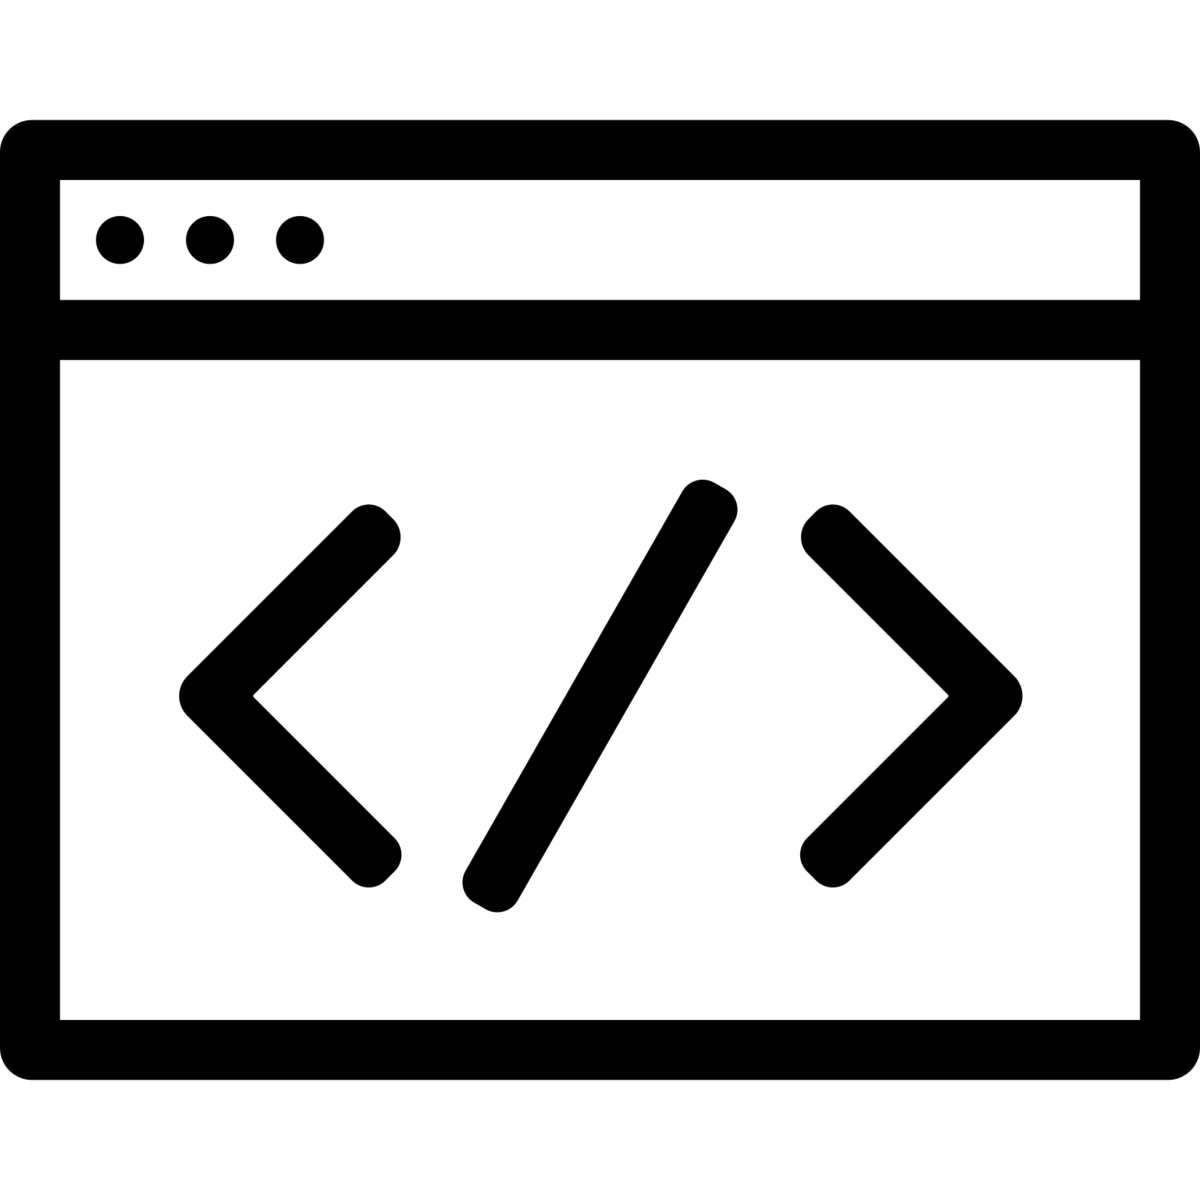
\includegraphics[width=2cm]{figures/srccode.png}};
    \node (srcLabel) [above=-0.3cm of sourceCode,visible on=<1->] {Source Code};
    \node (compiler) [right of=sourceCode, visible on=<1->] {
\includegraphics[width=1cm]{figures/c.png}};
    \node (compilerLabel) [above=-0.3cm of compiler, visible on=<1->] {CompCert};
    \node (outputCode) [right of=compiler, visible on=<1->] {
\includegraphics[width=2.5cm]{figures/binary.png}};
    \node (outputLabel) [above=-0.55cm of outputCode, visible on=<1->] {Machine Code};


    \draw [->, thick, visible on=<1->, shorten >= 0.6cm] (sourceCode) -- (compiler);
    \draw [->, thick, visible on=<1->, shorten <= 0.6cm] (compiler) -- (outputCode);
    \node[draw,line width=2pt, rounded corners=5pt, fit=(compiler)(compilerLabel)] {};

    \node (front) [visible on=<1->, below=0.5cm of sourceCode] {\Large Front};
    \node (frontbug) [below=1cm of front,visible on=<2->] {\color{magenta} 0 GCC, 10 LLVM};
    \node (frontbugc) [below=0cm of frontbug,visible on=<5->] {\color{cyan} 6 CompCert???};
    \node (middle) [right of=front, visible on=<1->] {\Large Middle};
    \node (middlebug) [below=1cm of middle,visible on=<2->] {\color{magenta} 49 GCC, 75 LLVM};
    \node (middlebugc) [below=0cm of middlebug,visible on=<4->] {\color{cyan} 0 CompCert};
    \node (back) [right of=middle, visible on=<1->] {\Large Back};
    \node (dummy) [below=0.4 of middle]{};
    \node (backbug) [below=1cm of back,visible on=<2->] {\color{magenta} 17 GCC, 74 LLVM};
    \node (backbugc) [below=0cm of backbug,visible on=<3->] {\color{cyan} 0 CompCert};

    \node (citation) [below=2cm of middle, visible on=<2->] {\bf (Yang
      et al., 2011)};

    \draw [dashed, gray, visible on=<1->, shorten >= 0.3cm, shorten <= 0.7cm] (compiler) -- (front);
    \draw [dashed, gray, visible on=<1->, shorten >= 0.3cm, shorten <= 0.7cm] (compiler) -- (back);

    \draw [->, thick, visible on=<1->, shorten >= 0.3cm, shorten <= 0.3cm] (front) -- (middle);
    \draw [->, thick, visible on=<1->, shorten <= 0.3cm, shorten >= 0.3cm] (middle) -- (back);
    \node[draw,line width=2pt, visible on=<1->, rounded corners=2pt, fit=(front)] {};
    \node[draw,line width=2pt, visible on=<1->, rounded corners=2pt, fit=(middle)] {};
    \node[draw,line width=2pt, visible on=<1->, rounded corners=2pt, fit=(back)] {};
    \node[draw,line width=2pt, visible on=<6->, rounded corners=2pt, color=cyan,
      fit=(middle)(back), inner xsep =0.5cm, inner ysep =0.5cm] (verifBox) {};
    \node[below=0.1cm, inner sep=0pt, visible on=<6->] at (verifBox.south) {\color{cyan} Verified};
  \end{tikzpicture}
  \end{center}

\end{frame}

\begin{frame}{A Web of Trust}
\begin{center}
  \tikzset{
    foo1/.style={draw=none,black,font=\large\bf,xshift=2cm,yshift=3.5cm},
    foo2/.style={draw=none,black,font=\large\bf,xshift=2cm,yshift=0.5cm},
    bar/.style={draw=black,thick,scale=4}
  }
  \begin{tikzpicture}
    \onslide<5->{\path (0,4) pic [bar, fill=CornflowerBlue]
    {piece={0.8}{0.8}{0}{0}} node[foo1]
      {Parsing};o}
    \onslide<4->{\path (0,0) pic [bar, fill=CarnationPink]
    {piece={0}{-0.8}{-0.8}{0}} node[foo2]
      {Binary Generation};}
    \onslide<3->{\path (4,4) pic [bar, fill=YellowGreen]
    {piece={0.8}{0}{0}{-0.8}} node[foo1]
      {Source Code};}
    \onslide<2->{\path (4,0) pic [bar, fill=Goldenrod]
    {piece={0}{0}{-0.8}{0.8}} node[foo2]
      {Distributed System};}

    % Images
    \onslide<5->{\path (1.7,6) node {
\includegraphics[width=2cm,height=2cm]{figures/pt.png}};}
    \onslide<4->{\path (1.7,2) node {
\includegraphics[width=2cm,height=2cm]{figures/binary.png}};}
    \onslide<3->{\path (6.2,6) node {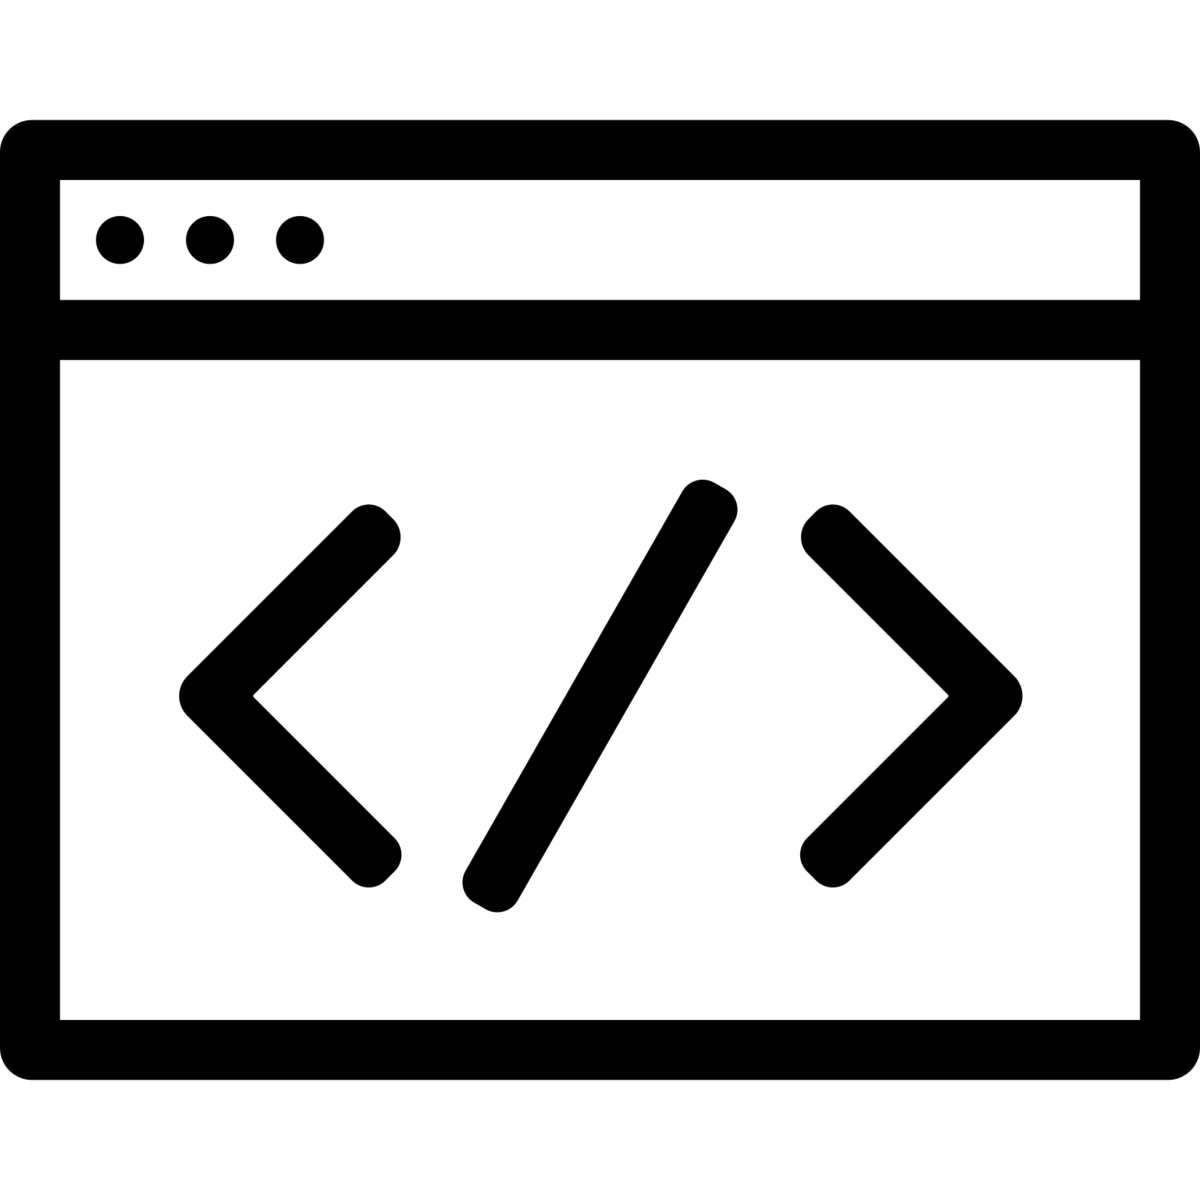
\includegraphics[width=2cm,height=2cm]{figures/srccode.png}};}
    \onslide<2->{\path (6.2,2) node {
\includegraphics[width=2cm,height=2cm]{figures/internet.png}};}
  \end{tikzpicture}
    \end{center}
\end{frame}

\begin{frame}{Validation of the CompCert Parser}
  CompCert parser rewritten and validated \textbf{(Jourdan et al, 2012)}
  \begin{itemize}
    \item<+-> Given a grammar and an automaton, validate that they agree
    \item<+-> Validator proven correct in Coq
    \item<+-> Generate a C parser with Menhir, then check correctness
  \end{itemize}

  \onslide<+->{Post-hoc verification takes time
  \begin{itemize}
    \item<+-> Requires more user input
    \item<+-> Harder to generalize
  \end{itemize}
  }
\end{frame}

\begin{frame}{Contributions of This Project}
  \begin{alertblock}{Goal}
    Build \textbf{correct-by-construction} parsers by means of type theory
  \end{alertblock}

  \onslide<2->{
  \begin{alertblock}{Roadmap}
    \begin{enumerate}
      \item<2-> Provide a type theory to reason about formal grammar theory
        \begin{itemize}
          \item<3-> Internalize existing ideas: Chomsky-style language theory,
                Kleene algebra, semantic actions, etc
        \end{itemize}
      \item<4-> Derive parser terms within the formalism
         \begin{itemize}
            \item<5-> Intrinsically verified by type system
         \end{itemize}
      \item<6-> Achieve an executable parser by embedding in Agda
    \end{enumerate}
  \end{alertblock}
  }
\end{frame}

\begin{frame}{Defining a Parser}
  \onslide<1->{\alert<1>{Input string $w$}} \qquad \onslide<2->{\alert<2>{Grammar $g$}}

  \onslide<3->{
  \begin{block}{\alert<3>{Parser Term}}
    $$ \alert<4>{w : \Sigma^{*}} \vdash \alert<7>{\mathsf{parse}_{g}(w)} : \alert<5>{g} \oplus \alert<6>{\top} $$
  \end{block}}

  \onslide<8->{
  \begin{exampleblock}{Example}
    \onslide<8->{\alert<8>{$g = a \otimes (b \oplus c)$}}

    \onslide<9->{\alert<9>{$w = ab$}}
    \onslide<10->{$\longrightarrow \mathsf{parse}_{g}(w) = {\color{cyan} \mathsf{inl}(p_{g})} : \alert<10>{g} \oplus \top$
    \quad {\LARGE \color{cyan} \cmark}}

    \onslide<11->{\alert<11>{$w = ad$}}
    \onslide<12->{$\longrightarrow \mathsf{parse}_{g}(w) = {\color{magenta} \mathsf{inr}(p_{\top})} : g \oplus \alert<12>{\top}$
    \quad {\LARGE \color{magenta} \xmark}}
  \end{exampleblock}}
\end{frame}

\section{Formal Grammars}

\begin{frame}{Formal Grammar Theory}
  A \emph{formal grammar} is a set of production rules for generating strings
  over an alphabet $\Sigma$ \pause
    \begin{itemize}
            \item A \emph{language} is a set of strings
    \end{itemize}

  \begin{exampleblock}{Same Number of $a$'s and $b$'s}
    $$L = \{ a^{n} b^{n} : n \geq 1 \}$$ \pause
    $L$ is generated by the grammar,
    \begin{align*}
      S & \to aSb \\
      S & \to ab
    \end{align*}
  \end{exampleblock}
\end{frame}

\begin{frame}{Chomsky Hierarchy}
  In the 50s, Chomsky gave a correspondence betweeen language classes and the machine that recognize them

  \begin{block}{Chomsky Hierarchy}
  \begin{center}
    \begin{tabular}{c c}
      \textbf{Language Class} & \textbf{Automata} \\
      Regular & Finite \\
      Context-free & Pushdown \\
      Context-sensitive & Linear-boundned \\
      Recursively-enumerable & Turing machine
    \end{tabular}
  \end{center}
  \end{block}
  \todoin{Animate this}
\end{frame}

\begin{frame}{Regular Expressions}
  \begin{itemize}
    \item<1-> The simplest grammars are regular
    \item<2-> Regular grammars can be induced from regular expressions
    \item<3-> Derive parsers for regular grammars, and later return to CFGs
  \end{itemize}
  \begin{center}
    \begin{tabular}{c c}
      \onslide<4->{ \alert<4>{Empty string}} &
                                               \onslide<4->{\alert<4>{$\varepsilon$}} \\
      \onslide<5->{ \alert<2>{Literal character}} &
                                                    \onslide<5->{\alert<5>{$c \in \Sigma$}} \\
      \onslide<6->{ \alert<6>{Concatenation}    } &
                                                    \onslide<6->{\alert<6>{$g \otimes h$}} \\
      \onslide<7->{ \alert<7>{Disjunction}      } &
                                                    \onslide<7->{\alert<7>{$g \oplus h$}} \\
      \onslide<8->{ \alert<8>{Kleene Star}      } & \onslide<8->{\alert<8>{$g^{*}$}} & \\ \\
      \onslide<9->{ \alert<9>{\textbf{Example}} } &
                                                    \onslide<9->{\alert<9>{$a^* \otimes (b \oplus c$)}}
    \end{tabular}
  \end{center}
\end{frame}

\begin{frame}{Parses of Regular Expressions}
  \begin{minipage}{.5\textwidth}
  $$g_{1} = {\color{cyan} a^{*}} \otimes ({\color{magenta} b} \oplus {\color{YellowOrange} c})$$
  \onslide<2->{$$w_{1} = aaab \to {\color{cyan}aaa}{\color{magenta}b} $$}
  \end{minipage}%
  \begin{minipage}{.5\textwidth}
  $$g_{2} = {\color{cyan} a^{*}} \otimes {\color{magenta}a^{*}}$$
  \onslide<3->{
  $$w_{2} = aaa \to {\color{magenta}aaa}, {\color{cyan}a}{\color{magenta}aa},
  {\color{cyan}aa}{\color{magenta}a},
  {\color{cyan}aaa}$$
  \onslide<4->{$$w_{3} = asdf \to \text{ rejected}$$}}
  \end{minipage}
  \todoin{layout slide, draw parse trees}
\end{frame}

\begin{frame}{Grammars as Functions}
  A \emph{grammar} $g$ is a function $g : \Sigma^{*} \to \Set$
  \begin{itemize}
    \item Strings are mapped to the set of parse trees matching $g$
  \end{itemize}

  \begin{minipage}{.5\textwidth}
  $$g_{1} = {\color{cyan} a^{*}} \otimes ({\color{magenta} b} \oplus {\color{YellowOrange} c})$$
  \onslide<2->{
  $$w_{1} = aaab$$
  $$g_{1}(w_{1}) = \{ {\color{cyan}aaa}{\color{magenta}b} \} $$
  }
  \onslide<3->{
  $$w_{2} = aaa$$
  $$g_{2}(w_{2}) = \{ {\color{magenta}aaa}, {\color{cyan}a}{\color{magenta}aa},
  {\color{cyan}aa}{\color{magenta}a},
  {\color{cyan}aaa} \}$$
  }
  \onslide<4->{
  $$w_{3} = asdf$$
  $$g(w_{3}) = \{\}$$
  }
  \end{minipage}
  \todoin{layout slide}
\end{frame}

\begin{frame}{Grammars as Presheaves}
  Grammar
  $g : \Sigma^{*} \to \Set$
  can be viewed as a functor

  \begin{itemize}
    \item<+-> $\Sigma^{*}$ viewed as a discrete category
    \item<+-> Functors into $\Set$ --- presheaves --- have significant structure
    \item<+-> Presheaves model dependent type theory
    \item<+-> Design a type theory where grammars are the intended model!
  \end{itemize}
\end{frame}

\begin{frame}{Grammars as Types}
  \begin{itemize}
    \item<+-> Capture grammar semantics natively via a type system
    \item<+-> Take inspiration from linear logic
      \begin{itemize}
        \item While parsing, characters of a string act as resources
      \end{itemize}
    \item<+-> Grammars are \textbf{types}, and parse trees are \textbf{terms}
  \end{itemize}

  \onslide<+->{
    \[
      \Delta \vdash M : g
    \]
  }
  \onslide<+->{
    \[
      x : g, y : h \vdash (x \otimes y) : g \otimes h
    \]
  }
  \onslide<+->{
    \[
      x : c, y : a, z : t \vdash (x \otimes y \otimes z) : c \otimes a \otimes t
    \]
  }
\end{frame}

\begin{frame}{(Lack of) Structural Rules}
  Omit these structural rules that usually appear in intuitionistic logic

  \begin{mathpar}
    \onslide<2->{
    \only<2>{\inferrule*[Right=Weakening]{\Delta \vdash M : g}{\Delta , x : A \vdash M : g}}
    \only<3->{\xcancel{\inferrule*[Right=Weakening]{\Delta \vdash M : g}{\Delta , x : A \vdash M : g}}}}

    \and

    \onslide<4->{

    \only<4>{\inferrule*[Right=Contraction]{\Delta , x : A , y : A \vdash  M : g}{\Delta , z : A \vdash
      M[ z / x , z / y ] : g}}
    \only<5->{\xcancel{\inferrule*[Right=Contraction]{\Delta , x : A , y : A \vdash  M : g}{\Delta , z : A \vdash
      M[ z / x , z / y ] : g}}}
     }

    \\

    \onslide<6->{
    \only<6>{\inferrule*[Right=Exchange]{\Delta , \Delta' \vdash M : g}{\Delta' , \Delta
      \vdash M : g}}
    \only<7->{\xcancel{\inferrule*[Right=Exchange]{\Delta , \Delta' \vdash M : g}{\Delta' , \Delta
      \vdash M : g}}}}
  \end{mathpar}

  \onslide<8->{Entire context must be used, \emph{exactly once} and in order}

  \onslide<9->{Just like when reading a word}
\end{frame}

\begin{frame}{Kleene Star}
  Take a least fixed-point operator $\mu$ as primitive

  \onslide<2->{
    Allows definition of recursive grammars
  }

  \onslide<3->{
    \[
      \inferrule{\Delta \vdash e : A[\mu x . A / x]}{\Delta \vdash \mathsf{cons}~e : \mu x . A}
    \]
  }
  \onslide<4->{
    \[
      g^{*} := \mu {\color{YellowOrange} x} . ({\color{cyan}\varepsilon} \oplus ({\color{magenta} g} \otimes {\color{YellowOrange} x}))
    \]
  }
  \onslide<5->{
    Inductive data type with constructors,
    \begin{itemize}
      \item<5-> ${\color{cyan} \bullet} \vdash \mathsf{nil} : g^{*}$
      \item<6->
            ${\color{magenta} x : g}, {\color{YellowOrange} y : g^{*}} \vdash \mathsf{cons}(x , y) : g^{*}$
    \end{itemize}
  }
\end{frame}

\begin{frame}{Kleene Star Elimination}
  Constructors
  \[
    {\color{cyan} \bullet \vdash \mathsf{nil} : g^{*}} \qquad {\color{magenta} x : g, y : g^{*} \vdash \mathsf{cons}(x , y) : g^{*}}
  \]
  \onslide<2->{
  Eliminator
  \[
      \inferrule*[Right=$*$Elim]
      {
        {\color{cyan} \bullet \vdash p_{\varepsilon} : h} \\
        {\color{magenta} x : g, y : h \vdash p_{*} : h}
      }
      {p : g^{*} \vdash \mathsf{fold}(p_{\varepsilon}, p_{*})(p) : h}
    \]
  }
  \onslide<3->{
    \begin{exampleblock}{Example}
      \[
      \inferrule
      {
        \onslide<4->{        \bullet \vdash \mathsf{nil : (ab)^{*}}} \\
        \onslide<5->{x : abab, y : (ab)^{*} \vdash p_{*} : (ab)^{*}}
      }
      {p : (abab)^{*} \vdash \mathsf{fold}(\mathsf{nil},p_{*})(p) : (ab)^{*}}
      \]
    \end{exampleblock}
  }
\end{frame}

\section{Automata}

\begin{frame}{Automata as Recognizers}
  $g = a^{*} \otimes (b \oplus c)$

  \only<1>{$w = aab$}
  \only<2-21>{\alert<21>{$\alert<7>{w} = \alert<8-10>{a} \otimes  \alert<11-13>{a} \otimes \alert<14-16>{b}
    \only<18-19>{\otimes \alert{\varepsilon}}$} \quad \only<21>{ {\Large \color{cyan} \cmark}}}
  \only<22->{\alert<30>{$ w = \alert<23-25>{a} \otimes \alert<26-28>{b} \otimes \alert<29>{b}$}
     \quad \only<30>{ {\Large \color{magenta} \xmark}}}

  \onslide<3->{
  \begin{center}
  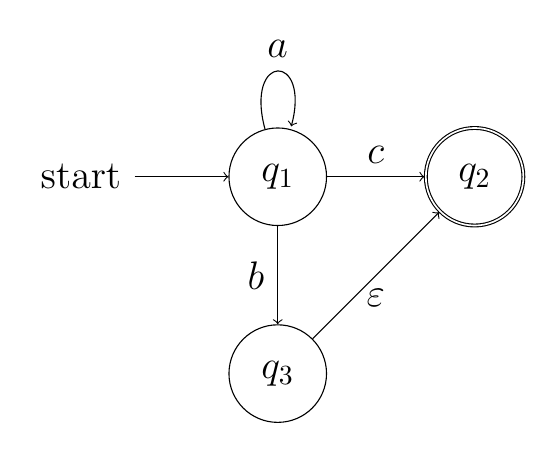
\begin{tikzpicture}[node distance = 25mm ]
    \Large
    \alert<4,8>{\node (0) {start};}
    \alert<4,8,10-11,13-14,23,25,26>{\node[state, right of=0] (1) {$q_{1}$};}
    \alert<5,20>{\node[state, right of=1, accepting] (2) {$q_{2}$};}
    \alert<16-17,28,29>{\node[state, below of=1] (3) {$q_{3}$};}

    \alert<15,27>{\draw[->] (1) edge[left] node{$b$} (3);}
    \draw[->] (1) edge[above] node{$c$} (2);
    \alert<9,12,24>{\draw[->] (1) edge[loop above] node{$a$} (1);}
    \alert<19>{\draw[->] (3) edge[below] node{$\varepsilon$} (2);}
    \alert<4,8>{\draw[->] (0) edge[above] node{} (1);}
  \end{tikzpicture}
  \end{center}}
\end{frame}

\begin{frame}{Automata as Grammars}
  $g = a^{*} \otimes (b \oplus c)$

  \onslide<2-21>{\alert<21>{$\alert<7>{w} = \alert<8-10>{a} \otimes  \alert<11-13>{a} \otimes \alert<14-16>{b}
    \only<18-19>{\otimes \alert{\varepsilon}}$} \quad \only<21>{ {\Large \color{cyan} \cmark}}}

  \onslide<3->{
  \begin{center}
  \begin{minipage}{.5\textwidth}
  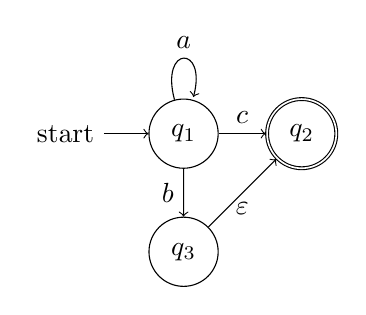
\begin{tikzpicture}[node distance = 15mm, scale=0.4]
    \alert<4,8>{\node (0) {start};}
    \alert<4,8,10-11,13-14>{\node[state, right of=0] (1) {$q_{1}$};}
    \alert<5,20>{\node[state, right of=1, accepting] (2) {$q_{2}$};}
    \alert<16-17>{\node[state, below of=1] (3) {$q_{3}$};}

    \alert<15>{\draw[->] (1) edge[left] node{$b$} (3);}
    \draw[->] (1) edge[above] node{$c$} (2);
    \alert<9,12>{\draw[->] (1) edge[loop above] node{$a$} (1);}
    \alert<19>{\draw[->] (3) edge[below] node{$\varepsilon$} (2);}
    \alert<4,8>{\draw[->] (0) edge[above] node{} (1);}
  \end{tikzpicture}
  \end{minipage}%
  \begin{minipage}{.5\textwidth}
    $$ \mathsf{Trace}(q_{1}, q_{2}) =$$
    \begin{equation*}
      \mu
      \begin{pmatrix}
        \alert<8,10,11,13,14>{g_{q_{1}}} := & \alert<9,12>{(a \otimes g_{q_{1}})} \\ & \oplus  ( c \otimes g_{q_{2}} ) \\ & \oplus \alert<15>{(b \otimes g_{q_{3}})} \\
        \alert<20>{g_{q_{2}}} := & \alert<5,20>{\varepsilon} \\
        \alert<16,17>{g_{q_{3}}} := & \alert<19>{g_{q_{2}}} \\
      \end{pmatrix}. \alert<4>{\color<21>{cyan} g_{q_{1}}}
    \end{equation*}
  \end{minipage}
  \end{center}}
\end{frame}

\begin{frame}{Accepting Traces of Automata}
    \begin{minipage}{.5\textwidth}
      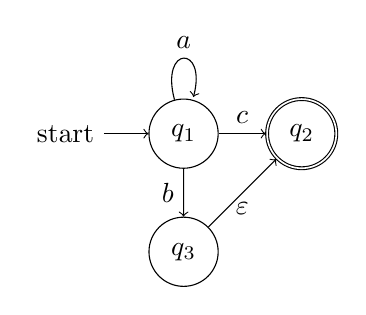
\begin{tikzpicture}[node distance = 15mm, scale=0.4]
        \node (0) {start};
        \node[state, right of=0] (1) {$q_{1}$};
        \node[state, right of=1, accepting] (2) {$q_{2}$};
        \node[state, below of=1] (3) {$q_{3}$};

        \draw[->] (1) edge[left] node{$b$} (3);
        \draw[->] (1) edge[above] node{$c$} (2);
        \draw[->] (1) edge[loop above] node{$a$} (1);
        \draw[->] (3) edge[below] node{$\varepsilon$} (2);
        \draw[->] (0) edge[above] node{} (1);
      \end{tikzpicture}
      \[ \mathsf{Trace}(\only<1>{q_{1}}\only<2->{\alert<2> {q_{2}}}, \only<1>{q_{2}}\only<2->{\alert<3>{q_{3}}}) \]
      \begin{equation*}
        \mu
        \only<1>{
        \begin{pmatrix}
          g_{q_{1}} := & (a \otimes g_{q_{1}}) \\ & \oplus  ( c \otimes g_{q_{2}} ) \\ & \oplus (b \otimes g_{q_{3}}) \\
          g_{q_{2}} := & \varepsilon \\
          g_{q_{3}} := & g_{q_{2}} \\
        \end{pmatrix}}\only<2->{
        \begin{pmatrix}
          g_{q_{1}} := & (a \otimes g_{q_{1}}) \\ & \oplus  ( c \otimes g_{q_{2}} ) \\ & \oplus (b \otimes g_{q_{3}}) \\
          g_{q_{2}} := & \alert<4>{\bot} \\
          g_{q_{3}} := & g_{q_{2}} \alert<3>{\oplus \varepsilon} \\
        \end{pmatrix}
        }. \only<1>{g_{q_{1}}}\only<2->{\alert<2>{g_{q_{2}}}}
      \end{equation*}
    \end{minipage}%
    \begin{minipage}{.5\textwidth}
      \onslide<5->{
      \[
        \mathsf{AccTrace} := \overline{\sum_{\alert<7>{q : Q}}} (\alert<8>{\mathsf{Trace}(q_{1}, q)}~\&~\alert<9>{\mathsf{acc}(q)})
      \]
      }
      \begin{itemize}
        \item<6-> An accepting trace is a triple\dots
        \begin{itemize}
          \item<7-> \alert<7>{An end state}
          \item<8-> \alert<8>{A trace starting at the initial state}
          \item<9-> \alert<9>{A proof that the end state is accepting}
        \end{itemize}
      \end{itemize}
    \end{minipage}%
\end{frame}

\begin{frame}{Deterministic Automata}
  A \emph{deterministic} finite automaton (DFA) has exactly one outgoing edge for every
  character $c \in \Sigma$ at every node

    \begin{minipage}{.5\textwidth}
      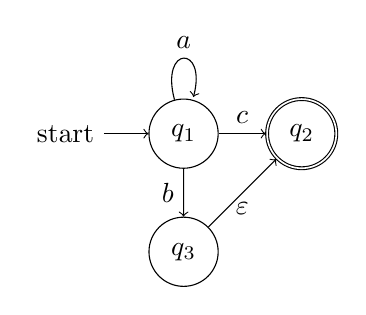
\begin{tikzpicture}[node distance = 15mm, scale=0.4]
        \node (0) {start};
        \node[state, right of=0] (1) {$q_{1}$};
        \node[state, right of=1, accepting] (2) {$q_{2}$};
        \node[state, below of=1] (3) {$q_{3}$};

        \draw[->] (1) edge[left] node{$b$} (3);
        \draw[->] (1) edge[above] node{$c$} (2);
        \draw[->] (1) edge[loop above] node{$a$} (1);
        \draw[->] (3) edge[below] node{$\varepsilon$} (2);
        \draw[->] (0) edge[above] node{} (1);
      \end{tikzpicture}
      \begin{center}
      \hspace{-1.5cm}
      \onslide<2->{ {\Huge \color{magenta} \xmark}}
      \end{center}
      \end{minipage}%
    \begin{minipage}{.5\textwidth}
      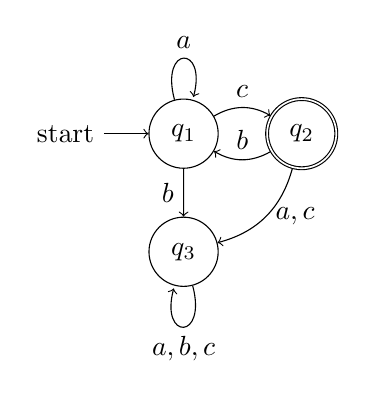
\begin{tikzpicture}[node distance = 15mm, scale=0.4]
        \node (0) {start};
        \node[state, right of=0] (1) {$q_{1}$};
        \node[state, right of=1, accepting] (2) {$q_{2}$};
        \node[state, below of=1] (3) {$q_{3}$};

        \draw[->] (1) edge[left] node{$b$} (3);
        \draw[->] (1) edge[above,bend left] node{$c$} (2);
        \draw[->] (2) edge[above,bend left] node{$b$} (1);
        \draw[->] (2) edge[right, bend left] node{$a,c$} (3);
        \draw[->] (1) edge[loop above] node{$a$} (1);
        \draw[->] (3) edge[loop below] node{$a,b,c$} (3);
        \draw[->] (0) edge[above] node{} (1);
      \end{tikzpicture}

      \begin{center}
      \hspace{-1.5cm}
      \onslide<3->{ {\Huge \color{cyan} \cmark}}
      \end{center}
      \end{minipage}
\end{frame}

\begin{frame}{Defining a Parser Term}
  $D$ a DFA grammar

  \[ w : \only<1>{\Sigma^{*}}\only<2->{\left( \bigoplus_{c \in \Sigma} c \right)^{*}} \vdash \mathsf{parse}_{D}(w) : \mathsf{AccTrace}_{D} \oplus \top \]

  \onslide<3->{Define with Kleene star eliminator!}

  \onslide<4->{
    \[
      A := \overline{\sum_{q : Q}} \mathsf{Trace}_{D}(q_{init}, q)
    \]
  \onslide<5->{
  \[
    \inferrule*[Right=$*$Elim]
    {
      \onslide<6->{\bullet \vdash p_{\varepsilon} : A} \\
      \onslide<7->{x : A, y : \left( \bigoplus_{c : \Sigma} c \right) \vdash p_{*} : A}
    }
    {w : \left( \bigoplus_{c \in \Sigma} c \right)^{*} \vdash M : A}
  \]}
  }
  \todoin{This slide is choppy and the bigoplus is confusing. Needs graphics}
\end{frame}

\begin{frame}{Results}
  \begin{itemize}
    \item<+-> We have a parser term for DFAs formalized in Agda
    \item<+-> We want a parser for regular expressions
    \item<+-> Prove that DFAs and regular expressions are equivalent to extend the DFA parser to a regular expression parser
  \end{itemize}
\end{frame}

\begin{frame}{Regular Expressions and Finite Automata}
  \begin{block}{Thompson's Construction (Formalized)}
    For every regular expression $g$, we may construct an NFA $N_{g}$ that is isomorphic to $g$.
  \end{block}

  \onslide<2->{
  \begin{block}{Determinization}
    For every NFA $N$, there is a DFA $D$ that recognizes the same language
  \end{block}}

  \onslide<3->{Combine the above to realize a regular expression parser}
\end{frame}

\begin{frame}{More Expressive Language Classes}
  \begin{itemize}
    \item Finite automata correspond to regular expressions
    \item<+-> Pushdown automata correspond to context free grammars
    \item<+-> Can apply analogous constructions to achieve a verified parser for
          (deterministic) context-free grammars
    \item<+-> Restricted forms of context sensitivity
  \end{itemize}
\end{frame}

\begin{frame}{Future Work}
  Grammar theory has advanced since the 60s
  \begin{itemize}
    \item<2-> Interval parsing grammars \textbf{(Zhang et al., 2023)}
    \item<3-> Binary data formats
  \end{itemize}

  \onslide<4->{There are other front end tasks}
  \begin{itemize}
    \item<5-> Semantic actions
    \item<6-> Typechecking
  \end{itemize}
\end{frame}

\begin{frame}{Related Work}
  \begin{itemize}
    \item<1-> CoStar \textbf{(Lasser et al., 2023)} gives a verified predictive
          parser for non-left-recursive context free grammars (CFGs)
    \item<2-> \textbf{(Danielsson, 2010)} gives a verified parser combinator library
          in Agda
      \begin{itemize}
        \item<3-> Verified parser for general CFGs
        \item<4-> \dots up to language equivalence
        \item<5-> Mentions ``normalization by evaluation'' and proofs as
              first-class objects
      \end{itemize}
  \end{itemize}
  \todoin{Less text, expand on Danielsson}
\end{frame}

\begin{frame}[standout]
  Questions?
\end{frame}

\end{document}
